% -----------------------------------------------------------------
% Document class: Article
\documentclass[ a4paper, twoside, 11pt]{article}
\usepackage{../../../macros-general}
\usepackage{../../../macros-article}
% Number of the handout, quiz, exam, etc.
\newcommand{\numero}{04}
\setcounter{numero}{\numero}

% -----------------------------------------------------------------
\begin{document}
\allowdisplaybreaks

\begin{center}
\Large Mec\'anica Vectorial (MECG-1001): Trabajo Aut\'onomo \numero \\[2ex]
\small \textbf{Semestre:} 2017-2018 T\'ermino II \qquad
\textbf{Instructor:} Luis I. Reyes Castro \qquad
\textbf{Paralelo:} 08
\end{center}
\fullskip

% =============================================
\begin{problem}
\textbf{[4 Puntos]} El bloque $B$ se mueve hacia abajo con una velocidad constante de 20 mm/s. En $t=0$, el bloque $A$ se mueve hacia arriba con una aceleraci\'on constante y su velocidad es de 30 mm/s. Si se sabe que en $t=3$ s el bloque deslizante $C$ se ha movido 57 mm a la derecha, determine \textit{(i)} la velocidad del bloque deslizante $C$ en $t=0$, y \textit{(ii)} las aceleraciones de los bloques $A$ y $C$. 

\begin{figure}[htb]
\centering
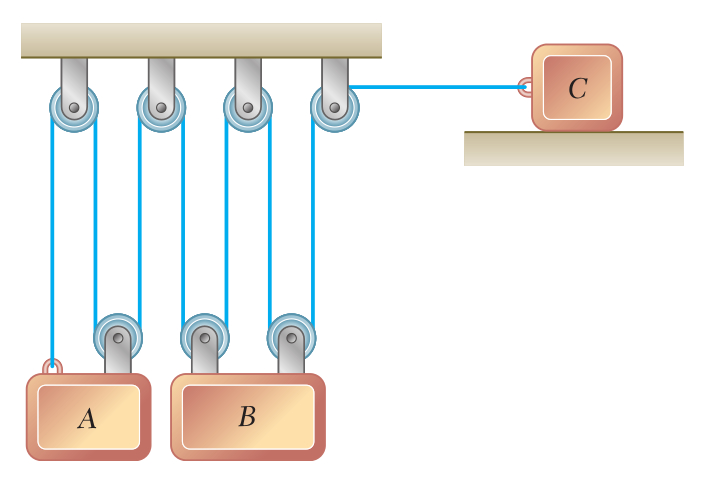
\includegraphics[width=0.5\textwidth]{problema-1.jpg}
\end{figure}

\end{problem}
\fullskip
\fullskip

% =============================================
\begin{problem}
\textbf{[4 Puntos]} Una puerta levadiza se gu\'ia mediante dos ruedas en $A$ y $B$ que giran sobre las correderas horizontal y vertical que se muestran en la figura. Si cuando $\theta = 40\deg$ la velocidad de la rueda $B$ es de 1.5 ft/s hacia arriba, determine \textit{(i)} la velocidad angular de la puerta y \textit{(ii)} la velocidad del extremo $D$ de la puerta. 

\begin{figure}[htb]
\centering
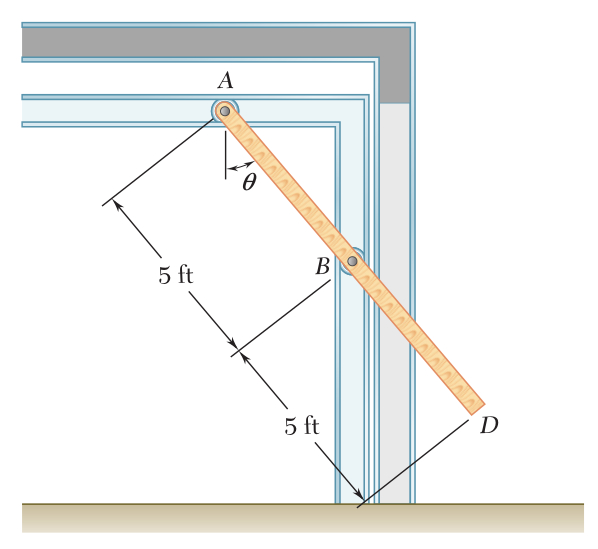
\includegraphics[width=0.5\textwidth]{problema-2.jpg}
\end{figure}

\end{problem}
\fullskip

\end{document}